\documentclass[12pt,parskip]{komatufte}
\usepackage[subpreambles=false]{standalone}

%%%%%%%%%%%%%%%%%%%%%%%%%%%
% Silence warning messages
\usepackage{silence}
\WarningsOff[scrlayer-notecolumn]
\WarningsOff[biblatex]

%%%%%%%%%%%%%%%%%%%%
% Commenting

%\usepackage[author=Lyndon]{pdfcomment}
%\newcommand{\pdfcomment}[1]{} %ignore all comments

%\usepackage{todonotes}
%\newcommand{\pdfcomment}{\todo}


%%%%%%%%%%%%%%%%%%%%
% Tables
\usepackage{booktabs}

%%%%%%%%%%%%%%%%%%%
% Fonts
\usepackage{tgadventor} %sans
\usepackage{tgpagella}  %serif
\usepackage{inconsolata} %mono
\usepackage[T1]{fontenc}

\usepackage{microtype}
\usepackage[all]{nowidow}
%%%%%%%%%%%%%%%%%%%%%%%
% Styling
\setcounter{secnumdepth}{4}
\setcounter{tocdepth}{2}

\usepackage{placeins}



%%%%%%%%%%%%%%%%%%%
% Math
\usepackage{amsmath, amssymb, stmaryrd, mathtools}
\DeclareMathOperator*{\argmin}{argmin}
\DeclareMathOperator*{\argmax}{argmax}

\usepackage{xparse,xstring,etoolbox}
% crossref this against notation section
\newcommand{\vv}[1]{\tilde{#1}} % vector
\newcommand{\seq}[1]{\mathcal{#1}} % sequence
\newcommand{\set}[1]{\mathbb{#1}} % set

%%%%%%%%%
% Indexing/sequence indexing
\newcommand{\seqind}[2]{#1^{#2}} % seqence index
\newcommand{\ind}[2]{#1_{#2}} % indexed
\newcommand{\disamb}[2]{#1^{\mathrm{#2}}} %disambiguated

%% Smart indexing and naming
\newcommand{\ifupper}[3]{
    \normalexpandarg
	\exploregroups
	\StrCount{ABCDEFGHIJKLMNOPQRSTUVWXYZ}{#1}[\uppercount]
	\ifnumgreater{\uppercount}{0}{#2}{#3}
}

%smart index
\DeclareDocumentCommand{\ii}{u{_} m}{
	\ifupper{#1}%
	{% just a single uppercase character, i.e. a matrix
		  %make sure the index is the right length
		\StrCount{#2}{,}[\indcount]
		\ifnumgreater{\indcount}{0}
		{ % Got multiple indexes so all good
		 	\ind{#1}{#2}
		}
		{ % Only 1 index so grab the column
		 	\ind{#1}{{:,#2}}
		}
	}%
	{% Not just a single upper case character
		\ind{#1}{#2}
	}
}

\DeclareDocumentCommand{\nn}{u{_} m}{
	\seqind{#1}{#2}
}

\DeclareDocumentCommand{\dd}{u{_} m}{
	\disamb{#1}{#2}
}

% Index of a vector
\DeclareDocumentCommand{\iv}{u{_} m}{\ii{\vv #1}_{#2}}
\DeclareDocumentCommand{\dv}{u{_} m}{\dd{\vv #1}_{#2}}
\DeclareDocumentCommand{\nv}{u{_} m}{\nn{\vv #1}_{#2}}

%exp
\let\oldexp\exp
\renewcommand{\exp}[1]{\oldexp \left( #1 \right)}
\newcommand{\exptwo}[1]{\oldexp_2 \left( #1 \right)}

\newcommand{\softmax}{\mathrm{smax}}

\DeclareMathOperator*{\expectedop}{\mathbb{E}}
\DeclareDocumentCommand{\expected}{u{_} m}{
	\expectedop\limits_{\mathrlap{#2}}
}

%%%%%%%%%%%%%%%%
%Graphics
\usepackage{tikz}
\usetikzlibrary{positioning, fit,  shapes.geometric}
\usepackage{ifthen}
\usepackage{etoolbox}

\tikzset{
	backgroundcolor/.style ={fill=white},
	every node/.append style={
		minimum height=7mm,
	},
	labe/.append style={
		%Blue,
		align = center,
		backgroundcolor,
		fill opacity=0.6,
		text opacity=1,
		font={\footnotesize\itshape}	
	},
	layer/.append style={
		draw,
		align = center,
		minimum height=7mm,
	},
	tight/.append style={
		inner sep=0.2mm,
	},
	lookupbox/.append style={
		draw=none,
		append after command={
		       	[shorten <= -0.5\pgflinewidth]
		       	([shift={(-1.5\pgflinewidth,-0.5\pgflinewidth)}]\tikzlastnode.north east)
		       	edge([shift={( 0.5\pgflinewidth,-0.5\pgflinewidth)}]\tikzlastnode.north west) 
		       	([shift={( 0.5\pgflinewidth,-0.5\pgflinewidth)}]\tikzlastnode.north west)
		       	edge([shift={( 0.5\pgflinewidth,-1.5\pgflinewidth)}]\tikzlastnode.south west)            
		       	([shift={( -1.5\pgflinewidth,+0.5\pgflinewidth)}]\tikzlastnode.south east)
		       	edge([shift={(-1.5\pgflinewidth,-0.5\pgflinewidth)}]\tikzlastnode.north east)
		},
		inner sep=0.7mm,
		outer sep=0mm,
		minimum width=25mm
	}
}

\usepackage{pgfplots}
\pgfplotsset{compat=1.14}
\pgfplotsset{sideplot/.append style={
		width=\notescolwidth,
		domain=-10:10,
		samples=101,
		smooth,
		enlarge y limits={abs=2},
		axis lines=middle,
		xlabel  = $z$,
		ylabel  = $y$,
	},
	equ/.append style={
		color=blue,
		thick,
		mark=none
	}
}

% Function  For a plot 
% it  needs to be declared in preamble because of how \makenote* interacts with multiple files
\def\errorsurface(#1,#2){(0.5*#1 + 0.7*#2 + sin(deg(1.5*#1 + #2^2)))^2}


\usepackage{graphicx}
\graphicspath{{./figs/}, {./}, {./figs/chaptersentencerrepr/}, {./figs/chapterintromachinelearning/}, {./figs/chapterwordrepr/}}
\usepackage{adjustbox}


%%%%%%%%%%%%%%%%%%%
% Refs
\usepackage{cleveref}

\addbibresource{master.bib}

%%%%%%%%%%%%%%%%%%%%
% Formatting

% for examples from natural language space.
\newcommand{\natlang}[1]{\ifmmode \text{``\texttt{#1}''} \else {``\texttt{#1}''}\fi}
% \ifmmode ``trick'' from https://tex.stackexchange.com/a/15194/5834

%%%%%%%%%%%%%%%%%%%%%


\begin{document}
	

\setchapterpreamble{%
	\dictum[J. M. G. ele Lammens, PhD Dissertation,
	\textit{A~Computational Model of Color Perception and Color Naming},  State University of New York, 1994]{%
Whether one sees the artificial neural network technique described below as learning or as optimization depends largely on one's background and one's theoretical likes and dislikes. I will freely use ``learning'' in the remainder of this section because that term is traditionally used in the neural networks literature, but the reader should feel free to substitute ``optimization'' if (s)he finds the other term offensive. Please contact the author for an Emacs lisp function to enforce the usage of choice.%
}}
\chapter{Introduction to neural networks for machine learning}\label{sec:machine-learning-for-representations}
\aside[Suggested Reading]{ As this is not a comprehensive introduction we recommend the reader to look elsewhere for additional reading.
In particular we recommend
the free online web-book: \citetitle{WebBookBackprop} \parencite{WebBookBackprop},
and the comprehensive: \citetitle{TheDeepLearningBook} \parencite{TheDeepLearningBook}.
}


\begin{abstract}
	This chapter covers the crucial machine learning techniques required to understand the remained of the book: namely neural networks.
	Readers already familiar with neural networks can freely skip this chapter.
	Readers interested in a more comprehensive coverage of all aspects of machine learning are referred to the many textbooks on this subject matter.
\end{abstract}

Machine learning, particularly neural networks, has become a hot topic in recent years.
The core notion of machine learning is to learn to perform a function based on examples.
This is in-contrast to ``regular programming'' where code is written to accomplish the function based on the programmer's analysis of the task.
Machine learning is at its most useful when it is difficult to articulate explicit rules for finding an output from a given input; but for which there are many examples of such.
For example, the rule of English spelling ``I before E, except after C'', is known to be often incorrect.
It is hard to write a rule about letter order.
However, a dictionary (or any other corpus) will have thousands of words showing the correct order.
By applying suitable machine learning techniques,
a system could learn to determine the correct spelling of words containing \natlang{ie} and \natlang{ei},
and inform the users as to if an input word is correct, even if the word never occurred in the training dictionary.
This is because the machine learning algorithm (ideally) discovers generalisable rules, from the training examples.
For most machine learning methods, including neural networks, these rules are not in a readily interpretable form, but are stored as numerical parameters of the model.
It is for this reason they are often called black-box models.



\section{Neural Networks}
\aside[Multilayer perceptron or Artificial Neural Network?]{An artificial neural network is sometimes called a multilayer perceptron.
This is in reference to the (distantly) related perceptron learning algorithm.
This term has generally fallen out of favour in newer works,
with Geoffrey Hinton, who originally coined the term, expressing his own regret at the naming.
Sometimes the term multilayer perceptron is used to distinguish feed-forward neural networks,
from other neural network related technologies,
such as restricted Boltzmann machines, Hopfield networks, self-organizing maps etc.
Unless otherwise specified, we use the term neural network to refer to a feed-forward network as discussed in this chapter.
}

A neural network is one particular family of machine learning algorithms.
It is important to understand that neural networks are not emulations of the brain,
they are algorithms that were inspired by the ideas about how the brain worked \pcite{hebb1949organization}.
Some advancements have also been inspired by the functioning of the brain,
but many others have come from statistical methods or elsewhere.
A neural network is no more similar to a brain, than it is to a Fourier transform.

The core idea behind a neural network is to represent the transformation of the input to the output as links between neurons in a sequence of layers.
Each neuron has a weighted connection to the neurons in the layer below,
and it applies a nonlinear function to this weighted sum, 
to determine its own output.
The output is connected to the inputs in the layer above, or is the final output.

\pdfcomment{Maybe a diagram and/or some equations here. and a bit more detail?}


\aside[Don't implement neurons]{
Typical object orientated programming teaches one to look for objects.
A obvious object in a neural network would be a neuron.
Another object could be the connection (weight).
Perhaps a different subclass of neuron would be for each activation function.
Do not do this.
It will be incredibly slow in almost any programming languages -- where objects are always stored by reference, thus requiring a pointer dereferencing for each operation on each neuron.
Object orientated is not a good paradigm for this kind of technical computing.
Instead program in terms of matrix's and vectors.
Potentially using objects for layers, or for the entire network.
This allows one to take advantage of efficient matrix algebra routines such as in BLAS and LAPACK.
}



\section{Function Approximation}
The Universal Approximation Theorem (UAT) tells us that a neural network can be used to approximate almost any function \parencite{mhaskar1992uat,leshno1993uat,SONODA2017uat}.
Here a function should be understood in the general sense -- classification is a function from observations to classes, regression is a function from observed values to target values.
More precisely, for any continuous bounded function,
the UAT states that there exists a neural network that can approximate that function, to any given degree of accuracy.
Further, it states that the network only needs a single hidden layer.
In a less rigorous sense, of approximation, such a continuous bounded function can approximate any function, over a restricted sub-domain of input values.

The earliest proofs of this was restricted to bounded activation functions like the sigmoid.
More recent work has extended this for unbounded activation functions like ReLU \pcite{SONODA2017uat}.

A network without any hidden layers is only able to approximate linear functions.
It is equivalent to a perceptron, or a linear SVM \parencite{backprop,minsky2017perceptrons}. 


However, the UAT does not tell us the values for those weight parameters,
nor does it promise that any method of training will ever reach them in finite time.
More significantly it does not inform as to how wide \emph{sufficiently wide} is,
nor if deeper is more efficient than wider.


\section{Network Hyper-parameters}
\aside[Hyper-parameters vs Parameters]{
	The weights and biases of the network are called its parameters.
	They are optimised during training.
	The other features of the network, including its topology, activation functions, and the training method (which often has its own set of options), are called the hyper-parameters. 
}

The key determination in applying neural networks to any problem,
is the choice of the hyper-parameters.
Including, the number of hidden layers, and their widths.
Neural networks can largely be thought of as black-boxes,
that can be trained to  accomplish tasks given a set of training examples.
Beyond recognising how to express the problem,
the choice of hyper-parameters is the most important decision when employing a neural network based solution.


\subsection{Width and Depth}
While the UAT has shown that a single hidden layer is sufficient,
it is not necessary optimal in terms of achieving best performance in practice.
For many problems it is better to have a deeper rather than wider network.
This realisation and the techniques to overcome issues relating to deeper networks lead the current deep learning trend.

\aside[What happened to Unsupervised Pretraining?]{
	\textcite{hinton2006fastDBN,bengio2007greedylayerwise} lead to a new resurgence of interests in neural networks.
	Pretraining with Deep Belief Networks allowed for deep networks to be trained.
	It was held for many years that it was necessary to use layer-wise unsupervised pretraining,
	even when one has only supervised data.
	\textcite{glorot2011deepRELUsparse} showed that with ReLU units, a deep network could be trained directly and achieve the same performance.
	As such unsupervised pretraining is now a more niche technique used primarily when there is an excess of unsupervised data.
}


In the last decade, deep nets have come back into fashion.
In brief the reasoning for this is a combination of a better techniques (e.g. ReLU, unsupervised pretraining),
better hardware (e.g. GPUs and Xeon Phi), and more labelled data (e.g. from crowd-sourcing platforms such as Amazon Mechanical Turk.)
This has allowed problems that were previously considered unsolvable with earlier shallow networks to be solved with deep networks achieving state of the art results.


The choice of the number of hidden layers (depth),
and the sizes (width) is a key parameter in designing a neural network.
It is arguably \emph{the} key parameter.
It can be assessed using a hyper-parameter sweep on a validation or development dataset.
It is a particularly relevant parameter for our purposes, as hidden layers normally are directly linked to our representations of natural language.


%\subsection{Connectivity}



\subsection{Activation functions}

\aside[Notation: Generic Activation Function $\varphi$:]{Though-out this book, when the activation function is not significant to the problem at hand, we will represent it with the \mbox{symbol $\varphi(\cdot)$.}}

The universal approximation theorem places a number of requirements on the choice of activation function.
These requirements have been progressively relaxed by works such as \textcite{leshno1993uat, SONODA2017uat}.
This section discusses the activation functions in common use today.

The choice of activation function determines the range of output of a neuron.
For the hidden layers these generally perform relatively similarly.
Sigmoid, tanh, and ReLU are the most common activation functions used for hidden layers.
The range of output of a hidden layer does not normally matter, as it is by definition hidden.
More significantly, the final activation function or the output function does always matter.
The output function should be chosen for the task at hand.
As will be discussed in \Cref{sec:rnn} this also has significance when designing gated neural network structures.

\aside[Activation functions summary:]{
\emph{identity}: \hfill range {$(\infty,\infty)$}\\
\emph{sigmoid}:  \hfill range {$(0,1)$}\\
\emph{softmax}:  \hfill range {$(0,1)$}\\
\emph{tanh}:     \hfill range {$(-1,1)$}\\
\emph{ReLU}:     \hfill range {$(0,\infty)$}\\
\emph{ReLU6}:    \hfill range {$(0,6)$}
}

Beyond determining the range of the output, its derivative also determines the behaviour during training via gradient descent based training methods.
This is significant for activation functions like ReLU and ReLU6 discussed in the following sections.

The activation functions, other than the softmax layer, are applied element-wise to vector inputs.
As such the scalar definitions are given here.
We write $y = \varphi(z)$, for $y$ being the output, and $z$ being the weighted input from the layer below.
To represent the whole layer including weights and biases we write:
\begin{equation}
\v y =\varphi(z) = \varphi(W \v x + \v b)
\end{equation}

\subsubsection{Identity (Affine/Linear)}
The most basic activation function is the identity.
To simply output the weighted sum of the inputs, without applying a non-linearity.
It is commonly used as an output function for regression tasks,
as it imposes no (additional) bounds.

\begin{equation}
\v y= \v z
\end{equation}

Often the use of the identity activation function will be described in terms of the whole layer, including the weight and bias.
The layer is often called an affine layer as it corresponds to an affine transformation of its input.
When the bias is fixed at zero, this is a linear transformation of the input.

\begin{equation}
\v y=W \v x + \v b
\end{equation}
In this equation $W$ and $\v b$ are a trained weight matrix and bias vector respectively,
and $\v x$ is the output of the layer below.

Using an affine output layer on-top of the hidden layers
allows the learned scaling and shifting of any of the other activation functions.
However, when this is not needed it increases the difficulty of training for no benefit.

Identity functions cannot be used as hidden layer activation functions.
A stack of affine layers simplifies to be equivalent to a single affine layer, which means that the network can only approximate linear functions.
A non-linearity is required.
This is what the other activation functions provide.


\subsubsection{Sigmoid}

\asidefig[The sigmoid function]{
\begin{tikzpicture}
\begin{axis}[sideplot, enlargelimits={rel=0.25}]
\addplot+[equ] {1/(1+exp(-x))};
\end{axis}
\end{tikzpicture}
}

Sigmoid is the classic neural network activation function.
\begin{equation}
y=\sigma(z)=\frac{1}{1+\exp{-z}}
\end{equation}
Sigmoid outputs values between zero and one.
If the network has a single output then this is a fuzzy boolean.
It can be used to classify into two categories.
It is sometimes referred to the logistic output function as it forms the basis of logistic regression.
(Conversely, sometimes the word sigmoid is used to refer to all functions of such an S shape.)

Note that this function has the property that, $\sigma(-z)=1-\sigma(z)$.
This means negating the input to the final sigmoid in a binary classification network,
is the same as switching which class is considered as true.


\aside[Multinomial logistic regression]{A neural network classifier with a softmax output layer is sometimes called a multinomial logistic regression network (especially if there are no hidden layers), or even just a logistic regression network.
	This can lead to some confusion with a sigmoid outputting network.
	However, the similarity can be understood by considering a softmax output layer with 2 classes.
	For $\v z = \left[\iv z_1, \iv z_2\right]$
	defining $v=\iv z_1 - \iv z_2$ \\
	A (binary) logistic classification using the same inputs can be written:
	$P(Y{=}1)=\sigma(v) = \frac{1}{1+\exp{\iv z_2 - \iv z_1}}$.
	
	The 2 class softmax formulation is:\\
	$\softmax(\v z)$\\
	\scalebox{0.95}{$=\left[\frac{\exp{\iv z_1}}{\exp{\iv z_1}+\exp{\iv z_2}},  \frac{\exp{\iv z_2}}{\exp{\iv z_1}+\exp{\iv z_2}} \right]$} \\
		$=\left[\frac{1}{1+\exp{\iv z_2 - \iv z_1}},  \frac{1}{\exp{\iv z_1 - \iv z_2}+1} \right]$\\
		$=\left[ \sigma(v),  \sigma(-v) \right]$\\
		$=\left[ \sigma(v),  1-\sigma(v) \right]$\\
		$=\left[P(Y{=}1), P(Y{=}2) \right]$
}

\subsubsection{Softmax}
The standard output activation function for multiclass classification is softmax.
Formally, training a so-called softmax classifier is regression to a class probability, rather than a true classifier as it does not return the class but rather a prediction of each class's likelihood.
We will use the terms interchangeably.

Defining the layer $\v y$ in terms of its elements,
recall that by our notation convention $\iv y_i$ is the $i$th element of the vector $\v y=\left[\iv y_1,\,\iv y_2,\,\ldots \iv y_n\right]$:
\begin{equation}
\iv y_i=\i {\left(\softmax(\v z)\right)}_i= \frac{\exp{\iv z_i}}{\sum_{j=1}^{j=N} \exp{\iv z_j}}
\end{equation}
$\v y$ is a vector of length $n$, where $n$ the number of classes in the classification.
\pdfcomment{Diagram might be nice here}

These elements have  values between zero and one, and sum to one.
They thus define a discrete probability mass function.

When used for classification $\v y_i$ gives the probability of being in class $i$.
\begin{equation}
P(Y=i\mid \v z) = \i {\left(\softmax(\v z)\right)}_i  = \iv y_i
\end{equation}


Softmax is a \emph{soft}, i.e. differentiable,  version of what could be called \emph{hard-max}.
In this conceptual hard-max function, the largest output is set to one, and the others set to zero.
It is non-differentiable and thus not suitable for use in a neural network.
In softmax the largest values is proportionally increased to be closest to one,
and the smallest to be closest to zero.

Further consideration of the softmax is given in \Cref{sec:softmax-and-bayes-theorem}.

\subsubsection{Tanh}
\asidefig[the tanh function]{
	\begin{tikzpicture}
	\begin{axis}[sideplot, enlargelimits={rel=0.25}]
	\addplot+[equ] {tanh(x)};
	\end{axis}
	\end{tikzpicture}
}

The hyperbolic tangent function is a  scaled and shifted sigmoid function.
Such that the outputs are restricted to be between $-1$ and $+1$.

\begin{equation}
y=\tanh(z)=\frac{\exp{2z}-1}{\exp{2z}+1}=2\sigma(2z)+1
\end{equation}


\subsubsection{ReLU}
\asidefig[The ReLU function]{
	\begin{tikzpicture}
	\begin{axis}[sideplot, enlarge y limits={abs=2}, enlarge x limits={abs=0.25}]
	\addplot+[equ] {max(0,x)};
	\end{axis}
	\end{tikzpicture}
}

The Rectified Linear Unit (ReLU) is a more recently popularized activation function \pcite{dahl2013reludropout}.
It comes from earlier neuroscience work \pcite{hahnloser1998piecewise}.
\begin{equation}
y=ReLU(z)=\max \left( 0, z \right)=\begin{cases}
z & 0\le z\\
0 & z<0
\end{cases}
\end{equation}
Values are restricted to be at non-negative.
As this function has derivative zero for $z<0$, once a unit is turned off, it is not turned back-on.
During gradient descent (see \Cref{sec:gradient-descent-and-back-propagation}) the derivative is used to modify the weights, as it is zero it the weights will never change once turned off.
This is commonly called the neuron dying.
Further to this, using (zero mean) random initialization this ensures that approximately half of all neurons in the layer will initially be dead due to being randomly initialised to output a negative value.
This results in sparse connections between the layers.
This has been found to be a good thing \pcite{glorot2011deepRELUsparse}.
ReLU is very commonly used as a hidden layer activation function for deep networks.
It also helps with the gradient vanishing and gradient exploding problems that occur in deep networks \parencite{glorot2011deepRELUsparse}.
\pdfcomment{I think maybe this whole section needs to be moved to after I have explained gradient descent?}


\subsubsection{RELU6}
\asidefig[The RELU6 function]{
\begin{tikzpicture}
\begin{axis}[sideplot,  xtick={-6,-3, 0,3,6}, ytick={-3, 0,3,6}, enlarge y limits={abs=2}]
\addplot[equ] {max(0,min(x,6))};
\end{axis}
\end{tikzpicture}
}


Closely related to ReLU is ReLU6 \pcite{krizhevsky2010convolutional}.
This is another linear unit the saturates at 0, but also at 6.
\begin{equation}
y=ReLU6(z)=\max \left(0, \min\left(6, z\right) \right) =  \begin{cases}
6 & 6<z\\
z & 0\le z\le6\\
0 & z<0
\end{cases}
\end{equation}
\aside[Why are we bringing up ReLU6?]{ReLU6 is one of the more obscure activation functions. As such it may seem a bizarre inclusion in this shorter introduction. However, we have found it surprisingly successful as an activation function, e.g. in the auto-encoder example which follows in \Cref{sec:bottle-necking-autoencoder}. It also nicely illustrates the flexibility and indeed arbitrariness in how activation functions can be defined.}

This has similar advantages to ReLU.
However, as well as units being able to die to zero, it can also die to positive.
The bounding at 6, rather than any other number is rather arbitrary -- particularly given scaling with the intervening affine layers.
The important point is that it is bound both above and below.
This greatly simplifies any proofs of theoretical capabilities of various networks.



\subsubsection{Other activation functions}

There are numerous other activation functions.
Most are of interest for use in hidden layers such as Leaky RELU, Softplus, ELU and many others.
For specialized tasks, other functions might be used, such as atan2 \pcite{WhiteRepresentingAnglesSE}.


\section{Training}
The process of training the network is the process of solving a very high dimensional, nonlinear, non-convex global optimization problem.

\aside[Evaluation function vs Loss function]{
	We must distinguished between two types of \emph{error function}.
	The \emph{evaluation function} is the metric we are truly trying to improve, this could be accuracy for classification, BLEU score for translation, F1 score for retrieval etc.
	It is applied to the whole system (which may be greater than just the neural network), and the system may be evaluated in different ways using different evaluations.
	As the evaluation is often not differentiable, a proxy for it which we call the \textbf{loss function} is used in training.
	For example, squared error for regression, or cross-entropy for classification.
	The loss function is applied to the output of the network during training to calculate the error between the network output for a given input, and the target output from the training example.
	The loss function is designed such that minimising the loss function also (ideally) results in the true evaluation function being optimised.
}

Finding the globally optimal solution to such a function is itself a very difficult problem.
Nonlinear and non-convex problems can have local minima that are not global optima.
This means they cannot guarantee to reach a global optima by gradient descent.
However, this does not pose an issue for most neural networks as finding the true global optima is not required, merely finding a \emph{good enough} set of weights to get a \emph{good enough} result.

To train the network one must find the values for the networks weight and bias parameters, such that the total loss function is minimized over the training set.

To define the training problems as an optimisation problem one first considers the loss function for a single training case.
For a target output $y$ and an actual output $\hat{y}$, (considering the scalar case) a loss function is defined $loss(y, \hat{y})$.
For example the squared error loss (sometimes called L2 loss, though that risks confusion with L2 weight penalty for regularisation) used in regression is defined by
\begin{equation}
SE(y, \hat{y})=(y-\hat{y})^2
\end{equation}
The cross-entropy loss used in binary classification is defined by
\begin{equation}
	CE(y, \hat{y})=-\left((1-y)\log (1-\hat{y}) + y\log (\hat{y})\right)
\end{equation}
The choice of loss function depends on the purpose of the network.

When network function ($f$) is composed into the loss function
the per training case loss is given by $loss(\v y, \v f(\v x,\tilde{P}))$.
$\v f(\v x,\tilde{P})$ is the function that executes some neural network, with weight and bias parameters all grouped into $\tilde{P}$, upon an input $\v x$ where the target output is $\v y$.

The total loss ($Loss$) is defined by taking the sum over the whole training set ($\seq{X}$) of input output pairs.
\begin{equation}
Loss(\tilde{P}, \seq X) = \sum_{\forall (\v x, \v y)\in\seq{X}} loss(\v y, \v f(\v x,\tilde{P}))
\label{equ:totalloss}
\end{equation}
\Cref{equ:totalloss} nothing but a nonlinear function to be minimised by adjusting the values of the weights and biases in $\tilde{P}$.
\pdfcomment{P is not in the notation section, maybe change to W}

This can be given to off-the-shelf  unconstrained nonlinear optimisation algorithms \pcite{Ngiam2011} such as L-BFGS  \parencite{nocedal1980updating}.
Alternatively, and more commonly, the loss and updated can be processed iteratively on sub-sets, called minibatches, of the training data at a time.
The extreme case of this is to update for every single training example -- this is called online training.
Updating on minibatches is generally preferred over updating per example as it results in less small ``noisy'' weight fluctuations which may prevent reaching local minima.
It is preferred over full-batch (on the whole training set) as the more frequent updates allow for faster learning \pcite{lecun2012efficient}.
Minibatch optimisation is often performed using algorithms specifically targeted at machine learning applications such as Adam \parencite{kingma2014adam}.
In either case, almost all optimizers used for neural networks rely on gradient descent.

\aside[AdaGrad, AdaDelta, and Adam]{
AdaGrad \parencite{AdaGrad}, AdaDelta \parencite{DBLP:journals/corr/abs-1212-5701} and Adam \parencite{kingma2014adam}
 are effectively successive versions of an optimisation algorithm, specifically targeted at the machine learning case.
These algorithms dynamically adapt the learning rate during training.
There are several other algorithms in the family, for example RMSprop.
In recent works, Adam is the most commonly used optimiser.
\textcite{DBLP:journals/corr/DauphinVCB15} presents another algorithm from this family,
and considers how the adaptive learning rate is related to the second order derivative,
which is the fundamental innovation in more traditional quasi-Newtonian methods (over first-order methods like plain gradient descent.).
}


\subsubsection{Gradient Descent and Back-propagation}\label{sec:gradient-descent-and-back-propagation}
\aside[Back-propagation vs Gradient Descent?]{%
	Formally speaking, back-propagation finds the gradients, and Gradient Descent uses those gradients to update the network parameters.
	However, the terms are often used interchangeably.
}


Gradient descent is the basis of most commonly used optimisers in machine learning.
In gradient descent based methods the derivatives of the loss function relative to the parameters are used to update those parameters.
The parameters in this case are the network weights and biases.
To calculate the gradients the back-propagation algorithm is used.

Back-propagation is simply a method of applying the well-known chain-rule of calculus to the neural network loss functions \pcite{backprop}.
It allows one to calculate:  $\frac{\partial Loss}{\partial{\i W_{i,j}}}$
for any weight (or bias) parameter $\i W_{i,j}$ in the network.
These partial derivatives can always be found as the overall loss function, including the network, is differentiable \footnote{Technically most networks are differentiable almost everywhere. For some functions like ReLU they have some single points of where the derivative is not defined. But the derivatives here can be forced to a known value.} (when using typical activation functions and loss functions).

Using these gradients the network parameters can thus be updated.
Updating the parameters to a new value in the direction of the gradient decreases the loss (for the right step size).
This means for each $W_{i,j} \in \tilde{P}$ updating its value according to the local gradient.
\begin{equation}
\i W_{i,j} \leftarrow \i W_{i,j} - \alpha \frac{\partial Loss}{\partial{\i W_{i,j}}}
\end{equation}
where $\alpha$ is an update step size, commonly called the learning rate.
The more advanced methods discussed earlier, such as Adam, and L-BFGS, are extensions along this core principle.

\def\errorsurface(#1,#2){(0.5*#1 + 0.7*#2 + sin(deg(1.5*#1 + #2^2)))^2}
\asidefig[A visualisation of a possible error (loss) surface. The arrow indicates a possible step from one set of parameters (weights) down to another set of parameters with lower loss, via gradient descent.\label{fig:errorsurface}]{
\begin{tikzpicture}
\begin{axis}
[width=0.85\notescolwidth,
enlargelimits,
tick align=inside,
domain=-1:3,
samples=25,
xlabel=$\i W_{1,1}$,
ylabel=$\i W_{2,1}$,
zlabel=$Loss$
]
\addplot3[surf]{\errorsurface(x,y)};
\pgfmathsetmacro{\startstep}{\errorsurface(0.5,0.5)}
\pgfmathsetmacro{\endstep}{\errorsurface(0.15,0.15)}
\draw[->, thick] (axis cs:0.5,0.5,\startstep) -- (axis cs:0.15,0.15,\endstep);
\end{axis}
\end{tikzpicture}
}


If one considers a plot with the loss given on the vertical axis,
and the values of the parameters as describing a position on the horizontal axes,
then gradient descent is moving that the parameter-point downward on that surface based on local estimate of the slope.
Such a plot is shown in \Cref{fig:errorsurface}
Most real networks have far more than 2 parameters, of-course, however the process of gradient decent remains the same.





\section{Some Examples of Common Neural Network Architectures}
\aside[These examples are available online]{For a practical introduction to the networks discussed here, worked examples of these network are available in the accompanying blog post at \url{http://white.ucc.asn.au/NNforNLPBook/NNexamples}.
	They are written in the Julia programming language, making use of the TensorFlow.jl package.
}

We will discuss more linguistically relevant neural networks in the following chapters.
However, to introduce the topic, we will give some basic examples.


\subsection{Classifier}\label{sec:classifier}
\aside[FashionMNIST]{is a new image classification benchmarking dataset \parencite{xiao2017/online}.
It is a task to classify images of shirts, shoes and bags etc.
It is an exact drop-in replacement for MNIST.
It was created to allow the same benchmarking scripts to be used;
while using a different data set.
This combats extremely high use of MNIST leading to implicit test set information leakage in the design of ML systems (where systems are base on systems which perform well on MNIST due to more of such systems being published.);
as well as being a more difficult task, thus allowing better discrimination between systems.
}

A classifier on the MNIST challenge is one of the most common introductory networks.
The MNIST dataset is a collection of images of hand written digits, which much be classified as to which digit they are.

A basic network to complete this task is is shown in \Cref{fig:mnistnetwork}.

\begin{figure}
	\caption{The structure of a simple classifier network for MNIST.}
	\label{fig:mnistnetwork}
	\documentclass{standalone}

\usepackage{tikz}
\usetikzlibrary{positioning, fit,  shapes.geometric}
\usepackage{ifthen}
\usepackage{etoolbox}

\tikzset{
	backgroundcolor/.style ={fill=white},
	every node/.append style={
		minimum height=7mm,
	},
	labe/.append style={
		%Blue,
		align = center,
		backgroundcolor,
		fill opacity=0.6,
		text opacity=1,
		font={\footnotesize\itshape}	
	},
	layer/.append style={
		draw,
		align = center,
		minimum height=7mm,
	},
	tight/.append style={
		inner sep=0.2mm,
	},
	lookupbox/.append style={
		draw=none,
		append after command={
		       	[shorten <= -0.5\pgflinewidth]
		       	([shift={(-1.5\pgflinewidth,-0.5\pgflinewidth)}]\tikzlastnode.north east)
		       	edge([shift={( 0.5\pgflinewidth,-0.5\pgflinewidth)}]\tikzlastnode.north west) 
		       	([shift={( 0.5\pgflinewidth,-0.5\pgflinewidth)}]\tikzlastnode.north west)
		       	edge([shift={( 0.5\pgflinewidth,-1.5\pgflinewidth)}]\tikzlastnode.south west)            
		       	([shift={( -1.5\pgflinewidth,+0.5\pgflinewidth)}]\tikzlastnode.south east)
		       	edge([shift={(-1.5\pgflinewidth,-0.5\pgflinewidth)}]\tikzlastnode.north east)
		},
		inner sep=0.7mm,
		outer sep=0mm,
		minimum width=25mm
	}
}

\begin{document}

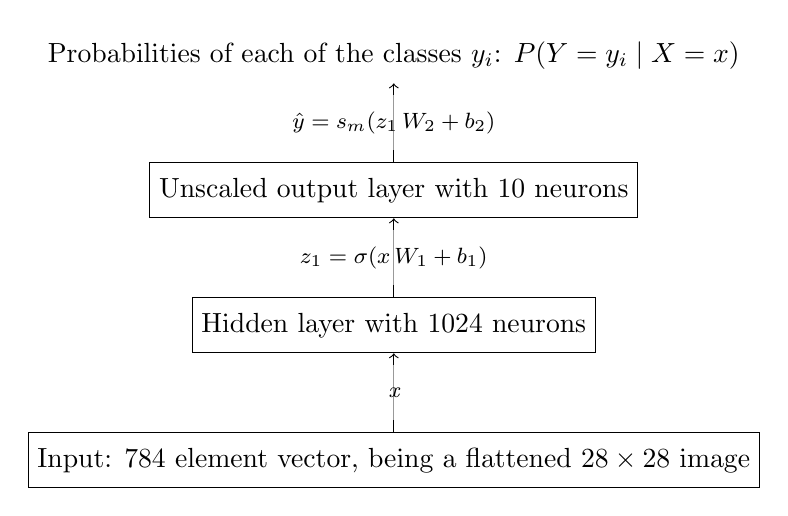
\begin{tikzpicture}[]

\node(in)[layer]{Input: 784 element vector, being a flattened $28 \times 28$ image};

\node(l1)[layer, above=of in]{Hidden layer with 1024 neurons};
\node(l2)[layer, above=of l1]{Unscaled output layer with 10 neurons};
\node(out)[above=of l2]{Probabilities of each of the classes $y_i$: $P(Y = y_i \mid X=x)$};

\draw[->] (in) edge  node[labe]{x} (l1);
\draw[->] (l1) edge  node[labe]{$z_1=\sigma(x\,W_1+b_1)$} (l2);
\draw[->] (l2) edge  node[labe]{$\hat{y}=s_m(z_1\,W_2+b_2)$} (out);

\end{tikzpicture}

\end{document}
\end{figure}

The network is defined by the equations:
\begin{align}
\v z&=\varphi(\d W_1 x + \dv b_1) \\
\hat{y}&=\softmax(\d W_2 z + \dv b_2) \\
P(Y{=}i{\mid}X{=}\v x) &= \hat{y}_i \\
&= \left[\softmax(\d W_2 \varphi(\d W_1 \v x + \dv b_1)+\dv b_2)\right]_i
\end{align}
for $X$ the input variable of grey-scale pixels intensities, and $Y$ the output as a class.
The output is represented with 1 hot encoding, where the index corresponding to the class is 1, and the others zero.


\aside[This simple network performs very well]{
	We note that this simple network can without further enhancement exceed the early published results for the MNIST challenge, using standard un-augmented neural networks,
	simply by using a very wide hidden-layer, that was not feasible at the time of those benchmarks.
	It is still outperformed by convolution neural networks and other better architectures.
}

To go into details about each layer:
The input is given by the grey scale pixel intensities in the original $28\times 28$ image.
This is flattened giving a $784$ element sized vector ($\v x$).
The first weight matrix projects that up onto a hidden layer  of width $1024$.
Thus $\d W_1$ is a $1024\times 784$ matrix.
The bias $\d {\v b}_1$ is for that hidden layer, so is a vector of length $1024$.
The hidden layer's actual activation values ($\v z$) for any input can be considered as being the values taken by 1024 different latent variables describing that input.
These are chosen  from a continuous abstract space of variables (via training) to effectively discriminate the correct class in the next layer (the output layer).

This is a shallow network, with only one hidden layer.
A deep network would have more hidden layers, for additional latent variables describing relations.
For the output layer we must project down to 10 dimensions, as there are 10 classes to choose from: the numbers from 0 to 9.
thus $\d W_2$ is a $10 \times 1024$ matrix,
and the bias $\dv b_2$ is a 10 element vector.
Using the softmax layer here ensures that output $\hat{y}$ is a valid probability mass function (nonnegative and summing to one).


\subsubsection{Softmax and Bayes' Theorem}\label{sec:softmax-and-bayes-theorem}
As a digression, it is worth considering the similarity between a network with a softmax output layer, and the application of Bayes' Theorem.
This will become important for understanding output embeddings, and hierarchical softmax in the future chapters.

The conditional probability of a classification given the value of some observed variable is defined by $P(Y=y\mid Z=\v z)$.
For $Y$ being the class taking value $i$;
and $Z$ the variable being conditioned upon, taking value $\v z$.
Here $\v z$  is some feature vector, this could be the output of a hidden layer below, or it could be a direct input.
Using softmax the estimated probability is given by
\begin{align} 
P(Y{=}i\mid Z{=}\v z) &= \i {\softmax(\v z)}_i\\
&=\frac{\exp{\i \left( W \v z+\v b\right)_{i}}}{\sum_{\forall j}\exp{\i \left( W \v z+\v b\right)_{j}}}\\
&=\frac{\exp{\i \left(W \v z \right)_{i}}\,\exp{\iv b_{i}}}{\sum_{\forall j}\exp{\i \left(W \v z\right)_{j}}\,\exp{\iv b_{j}}}
\end{align}

One can see that the bias term $\exp{\iv b_{i}}$ does not depend on the value of $z$.
The bias term is analogous to the prior probability.
Literally, it is the bias towards each element (i.e. each value $Y$ could take) without observing the condition.
We will define an unnormalised probability-like scoring function $R$;
and say $R(Y=i)=\exp{\iv b_{i}}$,
representing the marginal score contribution towards class $i$ from the bias.


The other component is $\exp{\i \left(W \v z \right)_{i}}$.
By considering this for each index $i$ (class value) that $Y$ might take then we have 
\begin{equation}
\i \left(W \v z \right)_{i}=\sum_{\forall j} \i W_{i,j} \, \iv z_{j} = \i W_{i,:} \v z
\end{equation}

Given one is considering the case for a particular class $Y=i$,
then it can be seen that the row vector $\i W_{i,:}$ as a weighting map for features possessed by $\v z$,
i.e. for input ($Z$) feature $j$, $\i W_{i,j}$ determines the relative weighting for that feature vs the other features of $Z$,
when the class is $i$.
When trained, the weight values should be such that it scores how likely the features are to occur for a given output class.
\pdfcomment{This sentence can be replaced wit ha stronger statement I think}

We can say that our scoring function $R$, has a likelihood term:
\begin{equation}
R(Z{=}\v z\mid Y{=}i)=\exp{\i \left(W \v z \right)_{i}}
\end{equation}

We will return to these row vectors  $\i W_{i,:}$ when we discuss as output embeddings in \Cref{sec:word-representations}.
$\i W_{i,:}$ must characterise the output class $i$, since difference classes would assign different importance to different features in the $Z$.
Furthermore, to some degree similar classes, i.e. classes triggered by similar features, would thus have more similar weights.


%
We can combine the unnormalised score factors to reformulate the original statement:
\begin{equation}
P(Y{=}i\mid Z{=}\v z)=\frac{R(Z{=}\v z\mid Y{=}i)\,R(Y{=}i)}{\sum_{\forall j}R(Z{=}\v z\mid Y{=}j)\,R(Y{=}j)}
\end{equation}


Contrast this to Bayes' Theorem:%
\aside[Marginal Denominator in Bayes Theorem]{In \Cref{eq:bayesmarginal}, notice that we replace $P(Z{=}\v z)$.
	We do this using the rule for finding marginal probabilities, from conditional probabilities with mutually exclusive and exhaustive condition values. This is always possible when working with classification.}%
%
\begin{align}
P(Y{=}i\mid Z{=}\v z)&=\frac{P(Z{=}\v z\mid Y{=}i)\,P(Y{=}i)}{P(Z{=}\v z)}\\
&=\frac{P(Z{=}\v z\mid Y{=}i)\,P(Y{=}i)}{\sum_{\forall j}P(Z{=}\v z\mid Y{=}j)\,P(Y{=}j)} \label{eq:bayesmarginal}
\end{align}



The similarities can be seen.
The bias effectively determines a prior probability-like term.
The weights defines the posterior probability: that is the chance of a particular class having a particular set of features.
The rows of the weight matrix mark how important each hidden feature is to each class. \pdfcomment{check rows vs cols}
We can consider that each row of the weight matrix is itself a representation of the class, as characterised by the importance of those latent features.
In the next chapter we will consider this as an output embedding.

A more traditional way of finding a representation of an input (rather than an output class) is to use an autoencoder.

\subsection{Bottlenecking Autoencoder}\label{sec:bottle-necking-autoencoder}

An autoencoder is a tool primarily used for finding a representation of their input.
There are many varieties of autoencoder based on neural network related techniques, including the works of \textcite{hinton2002RBM,hinton2006reducing,hinton2006fastDBN,vincent2010stacked,ICML2012Chen_416,2014VAE}.
This itself is a whole sub-field of machine learning.
Here we look at a simple bottlenecking autoencoder
\parencite{bourlard1988auto,japkowicz2000nonlinear}.
It has been used in a variety of tasks to attempt to find an optimal representation for an input e.g. as in \tcite{Usui:92}.
\begin{figure}
	\caption{A sampling of MNIST images from the test-set, arranged according to the values of 2 neurons on the encoding layer.}
	\label{mnist-encoding}
	\includegraphics[width=\textwidth]{figs/chapterintromachinelearning/mnist-encoding.png}
\end{figure}
An autoencoder is a neural network tasked with outputting its input.
This seemingly is a pointless task -- one already has the perfect reproduction of the input, in the input itself.
However, the true use of an autoencoder is to extract the output of one of the intermediary layers.
We call the intermediary layer the code layer.
To force this coded representation to have useful interesting properties,
and to prevent the network from simply learning the identity function,
all autoencoder include one or more features that increases the difficulty.
In the case of the bottlenecking autoencoder this feature is the bottleneck.
The code layer is much narrower than the input layer.
This forces the network to effectively learn to compress the data -- performing dimensionality reduction.

In this particular example we are looking at an auto-encoder for the MNIST images discussed earlier.
The original images are $28 \times 28$ pixels, i.e. 784 dimensional.
We compress it down to just 2 dimensions using the network shown in \Cref{fig-autoencoder}.

\begin{figure}
	\caption{A structure for a Bottle Necking Autoencoder for use on MNIST.}
	\label{fig-autoencoder}
	\resizebox{\textwidth}{!}{\documentclass{standalone}

\usepackage{tikz}
\usetikzlibrary{positioning, fit,  shapes.geometric}
\usepackage{ifthen}
\usepackage{etoolbox}

\tikzset{
	backgroundcolor/.style ={fill=white},
	every node/.append style={
		minimum height=7mm,
	},
	labe/.append style={
		%Blue,
		align = center,
		backgroundcolor,
		fill opacity=0.6,
		text opacity=1,
		font={\footnotesize\itshape}	
	},
	layer/.append style={
		draw,
		align = center,
		minimum height=7mm,
	},
	tight/.append style={
		inner sep=0.2mm,
	},
	lookupbox/.append style={
		draw=none,
		append after command={
		       	[shorten <= -0.5\pgflinewidth]
		       	([shift={(-1.5\pgflinewidth,-0.5\pgflinewidth)}]\tikzlastnode.north east)
		       	edge([shift={( 0.5\pgflinewidth,-0.5\pgflinewidth)}]\tikzlastnode.north west) 
		       	([shift={( 0.5\pgflinewidth,-0.5\pgflinewidth)}]\tikzlastnode.north west)
		       	edge([shift={( 0.5\pgflinewidth,-1.5\pgflinewidth)}]\tikzlastnode.south west)            
		       	([shift={( -1.5\pgflinewidth,+0.5\pgflinewidth)}]\tikzlastnode.south east)
		       	edge([shift={(-1.5\pgflinewidth,-0.5\pgflinewidth)}]\tikzlastnode.north east)
		},
		inner sep=0.7mm,
		outer sep=0mm,
		minimum width=25mm
	}
}

\begin{document}

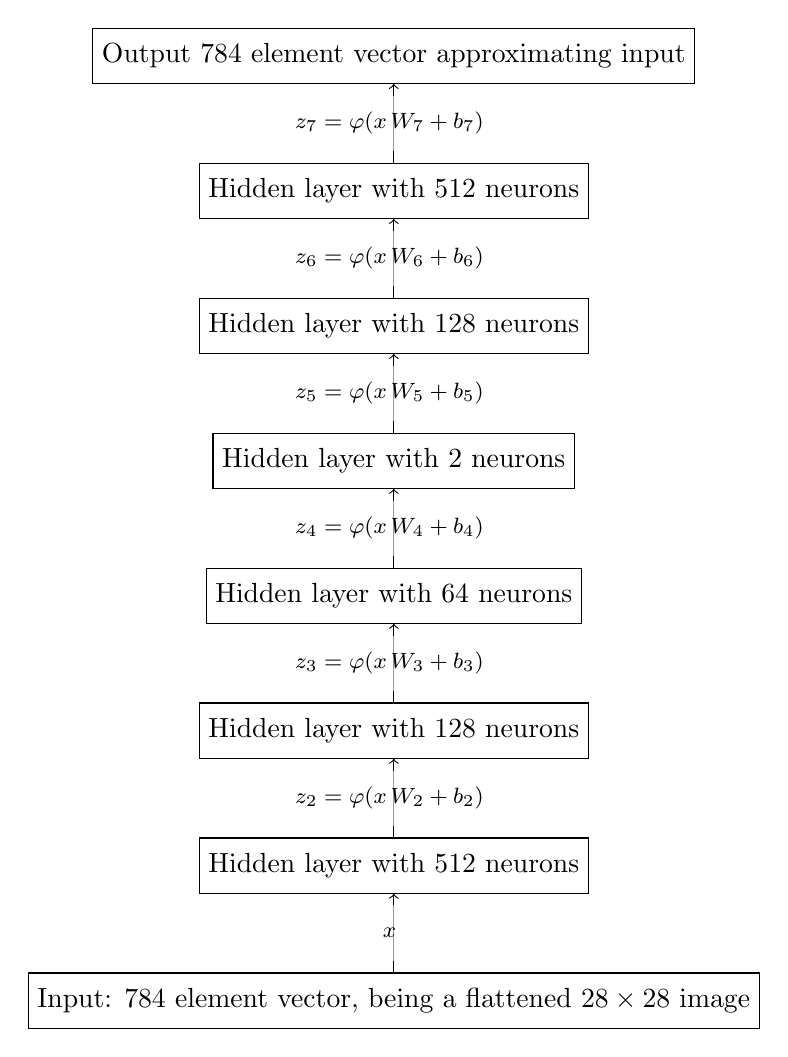
\begin{tikzpicture}[]

\node(L0)[layer]{Input: 784 element vector, being a flattened $28 \times 28$ image};

\foreach \i/\y[count=\j from 0] in {1/512, 2/128, 3/64, 4/2, 5/128, 6/512, 7/784}{
	\node(L\i)[layer, above= of L\j] {
		\ifthenelse{\j=6}{Output 784 element vector approximating input}%
		{Hidden layer with $\y$ neurons}%
	};
%
	\draw[->] (L\j) edge  node[labe]{
		\ifthenelse{\j = 0}{$x$}{$z_\i=\varphi(x\,W_\i+b_\i)$}
	}(L\i);	
}

%
\end{tikzpicture}

\end{document}}
\end{figure}

\FloatBarrier
In this particular network $\varphi$ is a leaky RELU6 unit.
\asidefig[The Leaky ReLU6 function. The leak level on this plot is exaggerated for purposes of visualisation.]{
	\begin{tikzpicture}
	\begin{axis}[sideplot,  xtick={-6, 0,6}, ytick={-3, 0,3,6}, enlarge y limits={abs=2}]
	\addplot+[equ] {max(0.05*x, min(1.05*x, 0.05*x + 6))};
	\end{axis}
	\end{tikzpicture}
}
\begin{equation}
\varphi(z)=\begin{cases}
    0.01z+6 & 6<z \\
	1.01z & 0 \le z \le 6 \\
	0.01z & z < 0
\end{cases}
\end{equation}

The reason for this is that a sigmoidal unit does not perform well in a deep network because of the gradient-vanishing/exploding effects.
As a result, only the bias information of the final layer mattered, effectively making all outputs just the average of all inputs.
The normal solution to this in deep networks is ReLU or ReLU6 units.

However, a ReLU, or ReLU6 unit is not ideal either,
as these units turn-off, and cannot turn back on again.
If one of the only 2 neurons in the code layer turn-off then they cannot turn back on again -- thus forcing it down to just one neuron, or none if that neuron also dies.
In trialling this network structure, this was found to occur quiet very often.

The solution was to add a ``leak'' to the unit.
A small constant gradient even in the saturated position.
Making such a neuron possible, even if difficult, to turn back on once turned off.
With this change the network always produces quality results.
An example of the recreation of an input from the test set can be seen in 
 \Cref{fig-ae-recreation}. 
It can be seen that the blur suggests that the input is a 7 or 9 like shape -- that level of information survived being squeezed through the bottleneck.


\asidefig[Recreation of an input from the MNIST test set. Input is on the left, output is on the right. 	{\label{fig-ae-recreation}}]{\includegraphics[scale=0.30]{figs/chapterintromachinelearning/recreation}}


More significantly, a sampling of the code layer is visually shown in \Cref{mnist-encoding}.
In this image, the positions on the X and Y axis for each input image is given by the values from the code layer for the representation of that image.
It can be seen that the code is capturing key information about the appearance.
The 0s appear near to the similarly rounded 6s,
the 8s near the 3s, etc.
In particular the 1s are arrayed according to their slope.
The autoencoder has captured very useful information about the inputs, that would be hard to define with any hand-written feature extractor.

It is this property of networks, to implicitly discover and define the most important latent variables and relationships to the task at hand that also makes it valuable for natural language processing.


\end{document}